\section{Modélisation et impression 3D}

Afin de permettre une intégration mécanique adaptée de la carte ST200 et de l’antenne KCM4, ainsi que la mise en œuvre de différents scénarios expérimentaux, plusieurs pièces mécaniques spécifiques ont été conçues et réalisées par impression 3D. Ces éléments constituent un support essentiel à la reproductibilité des essais et à la maîtrise de la géométrie d’acquisition.

\subsection{Conception des pièces mécaniques}

La conception des supports mécaniques a été réalisée à l’aide du logiciel de CAO \textit{Fusion~360} avec une licence étudiante. Cet environnement de modélisation a permis de concevoir des pièces sur mesure, directement adaptées à la géométrie de la carte ST200 et aux contraintes d’intégration de l’antenne radar.

Les pièces développées servent à deux choses. D’une part, elles assurent une fixation mécanique rigide et reproductible de l’antenne sur la carte ST200, tout en permettant un contrôle précis de l’angle d’installation de l’antenne, paramètre critique pour la géométrie d’illumination et la répétabilité des mesures. D’autre part, elles facilitent le montage de l’ensemble sur différents dispositifs expérimentaux, notamment un bras robotisé, afin de permettre des acquisitions dans des configurations variées et contrôlées.

Afin  de répondre au mieux aux besoins définis plus tôt une conception sous forme de boite à été réalisée.
On retrouve deux pièces dans laquelle la carte ST200 vient se fixer avant de venir y ajouter une pièce permettant de solidariser l'antenne au montage avec le tilt voulu. 
La modélisation 3D réalisé est la suivante : 

\begin{figure}[H]
    \centering
    
    \begin{subfigure}[t]{0.48\textwidth}
        \centering
        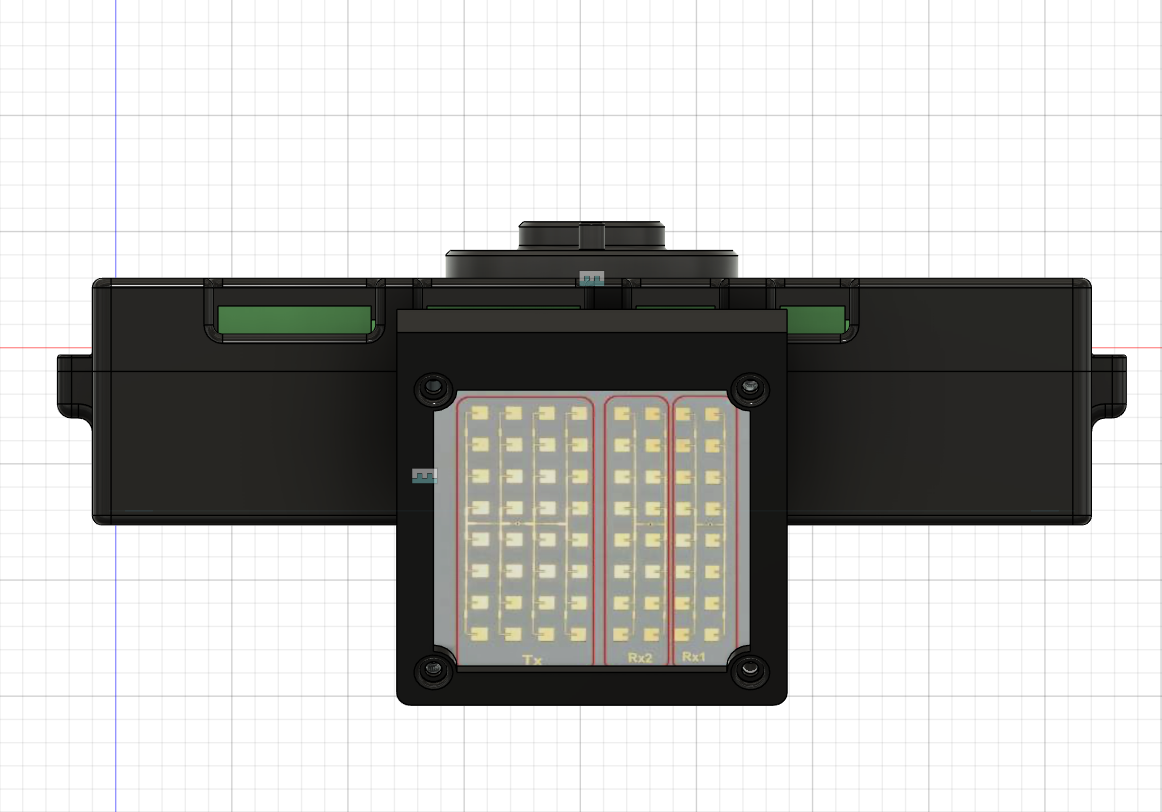
\includegraphics[width=\textwidth]{src/rapport_complet/img/Sardine_casing_face.png}
        \caption{Vue de la conception de face}
        \label{fig:Sardine_casing_face}
    \end{subfigure}
    \hfill
    \begin{subfigure}[t]{0.48\textwidth}
        \centering
        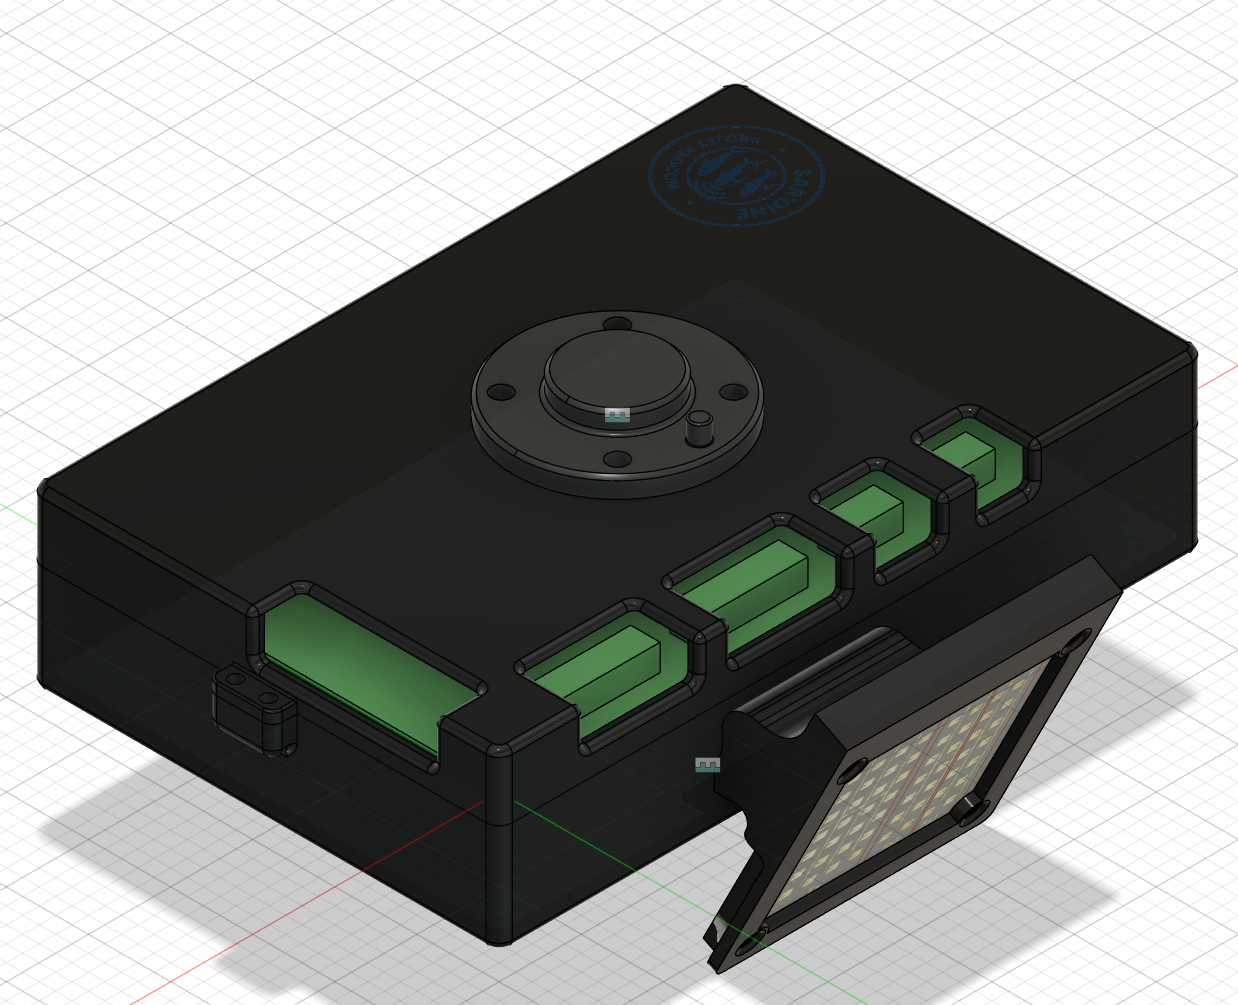
\includegraphics[width=\textwidth]{src/rapport_complet/img/SARDINE_CASING.png}
        \caption{Vue de la conception 3/4 plongeante }
        \label{fig:SARDINE_CASING}
    \end{subfigure}
    
    \caption{Modélisation 3D conçue}
    \label{fig:figure_globale}
\end{figure}

\subsection{Fabrication par impression 3D}

Les modèles issus de la phase de conception ont ensuite été exportés et fabriqués par impression 3D à l’aide des imprimantes 3D du FabLab de l'école. L’impression 3D a permis de produire des pièces à la fois légères et suffisamment rigides pour les essais réalisés, tout en maintenant un coût de fabrication et des délais réduits. Cette approche s’est révélée particulièrement adaptée au contexte expérimental du projet, où des ajustements de la géométrie mécanique étaient nécessaires pour répondre aux contraintes imposées par les protocoles de test (par exemple l'angle apporté à l'antenne).
Une fois les pièces imprimées nous avons pu réaliser l'assemblage des différentes parties et installer notre setup sur le bras robot en vue des premiers tests en mouvements: 

\begin{figure}[H]
    \centering
    
    \begin{subfigure}[t]{0.45\textwidth}
        \centering
        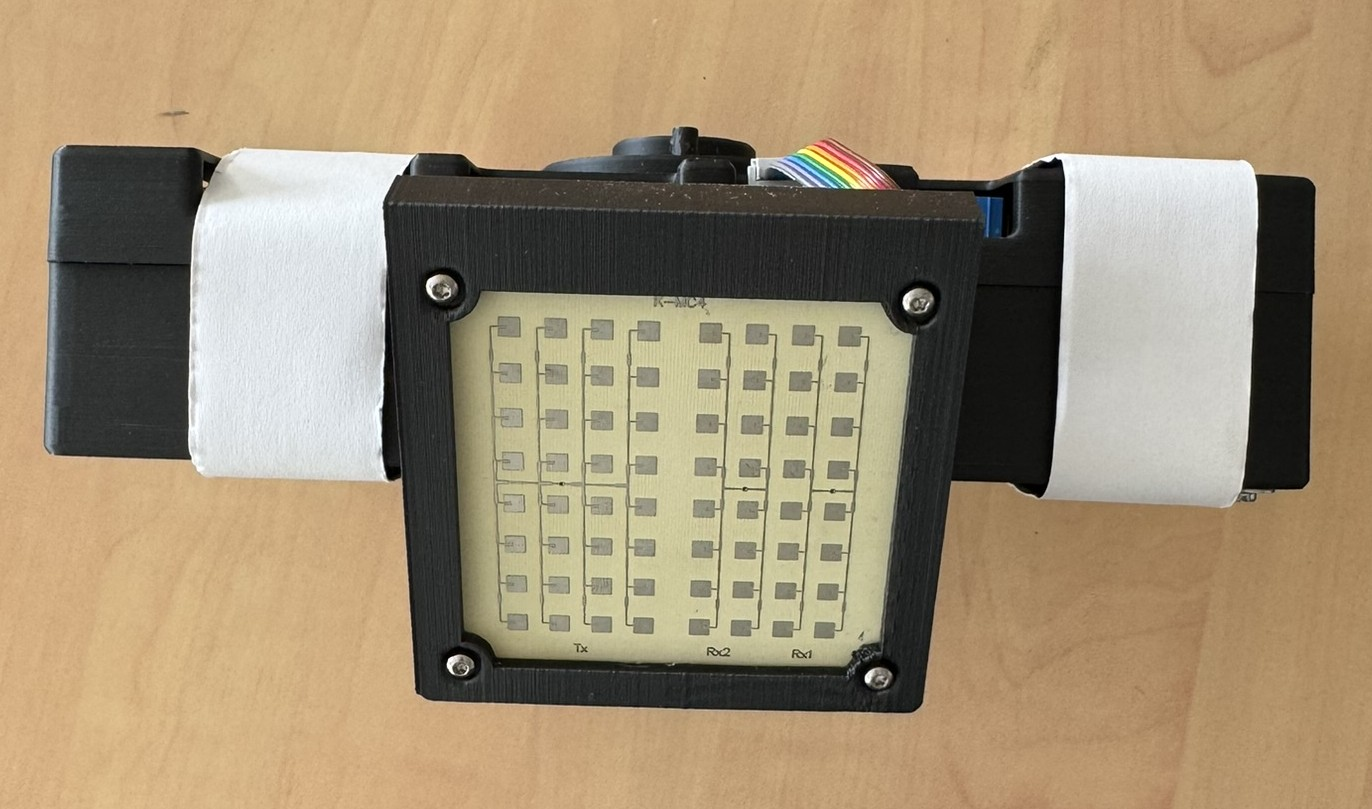
\includegraphics[width=\textwidth]{src/rapport_complet/img/Vue_casing_face.JPEG}
        \caption{Vue de l'assemblage de face}
        \label{fig:Sardine_casing_face}
    \end{subfigure}
    \hspace{0.05\textwidth}
    \begin{subfigure}[t]{0.45\textwidth}
        \centering
        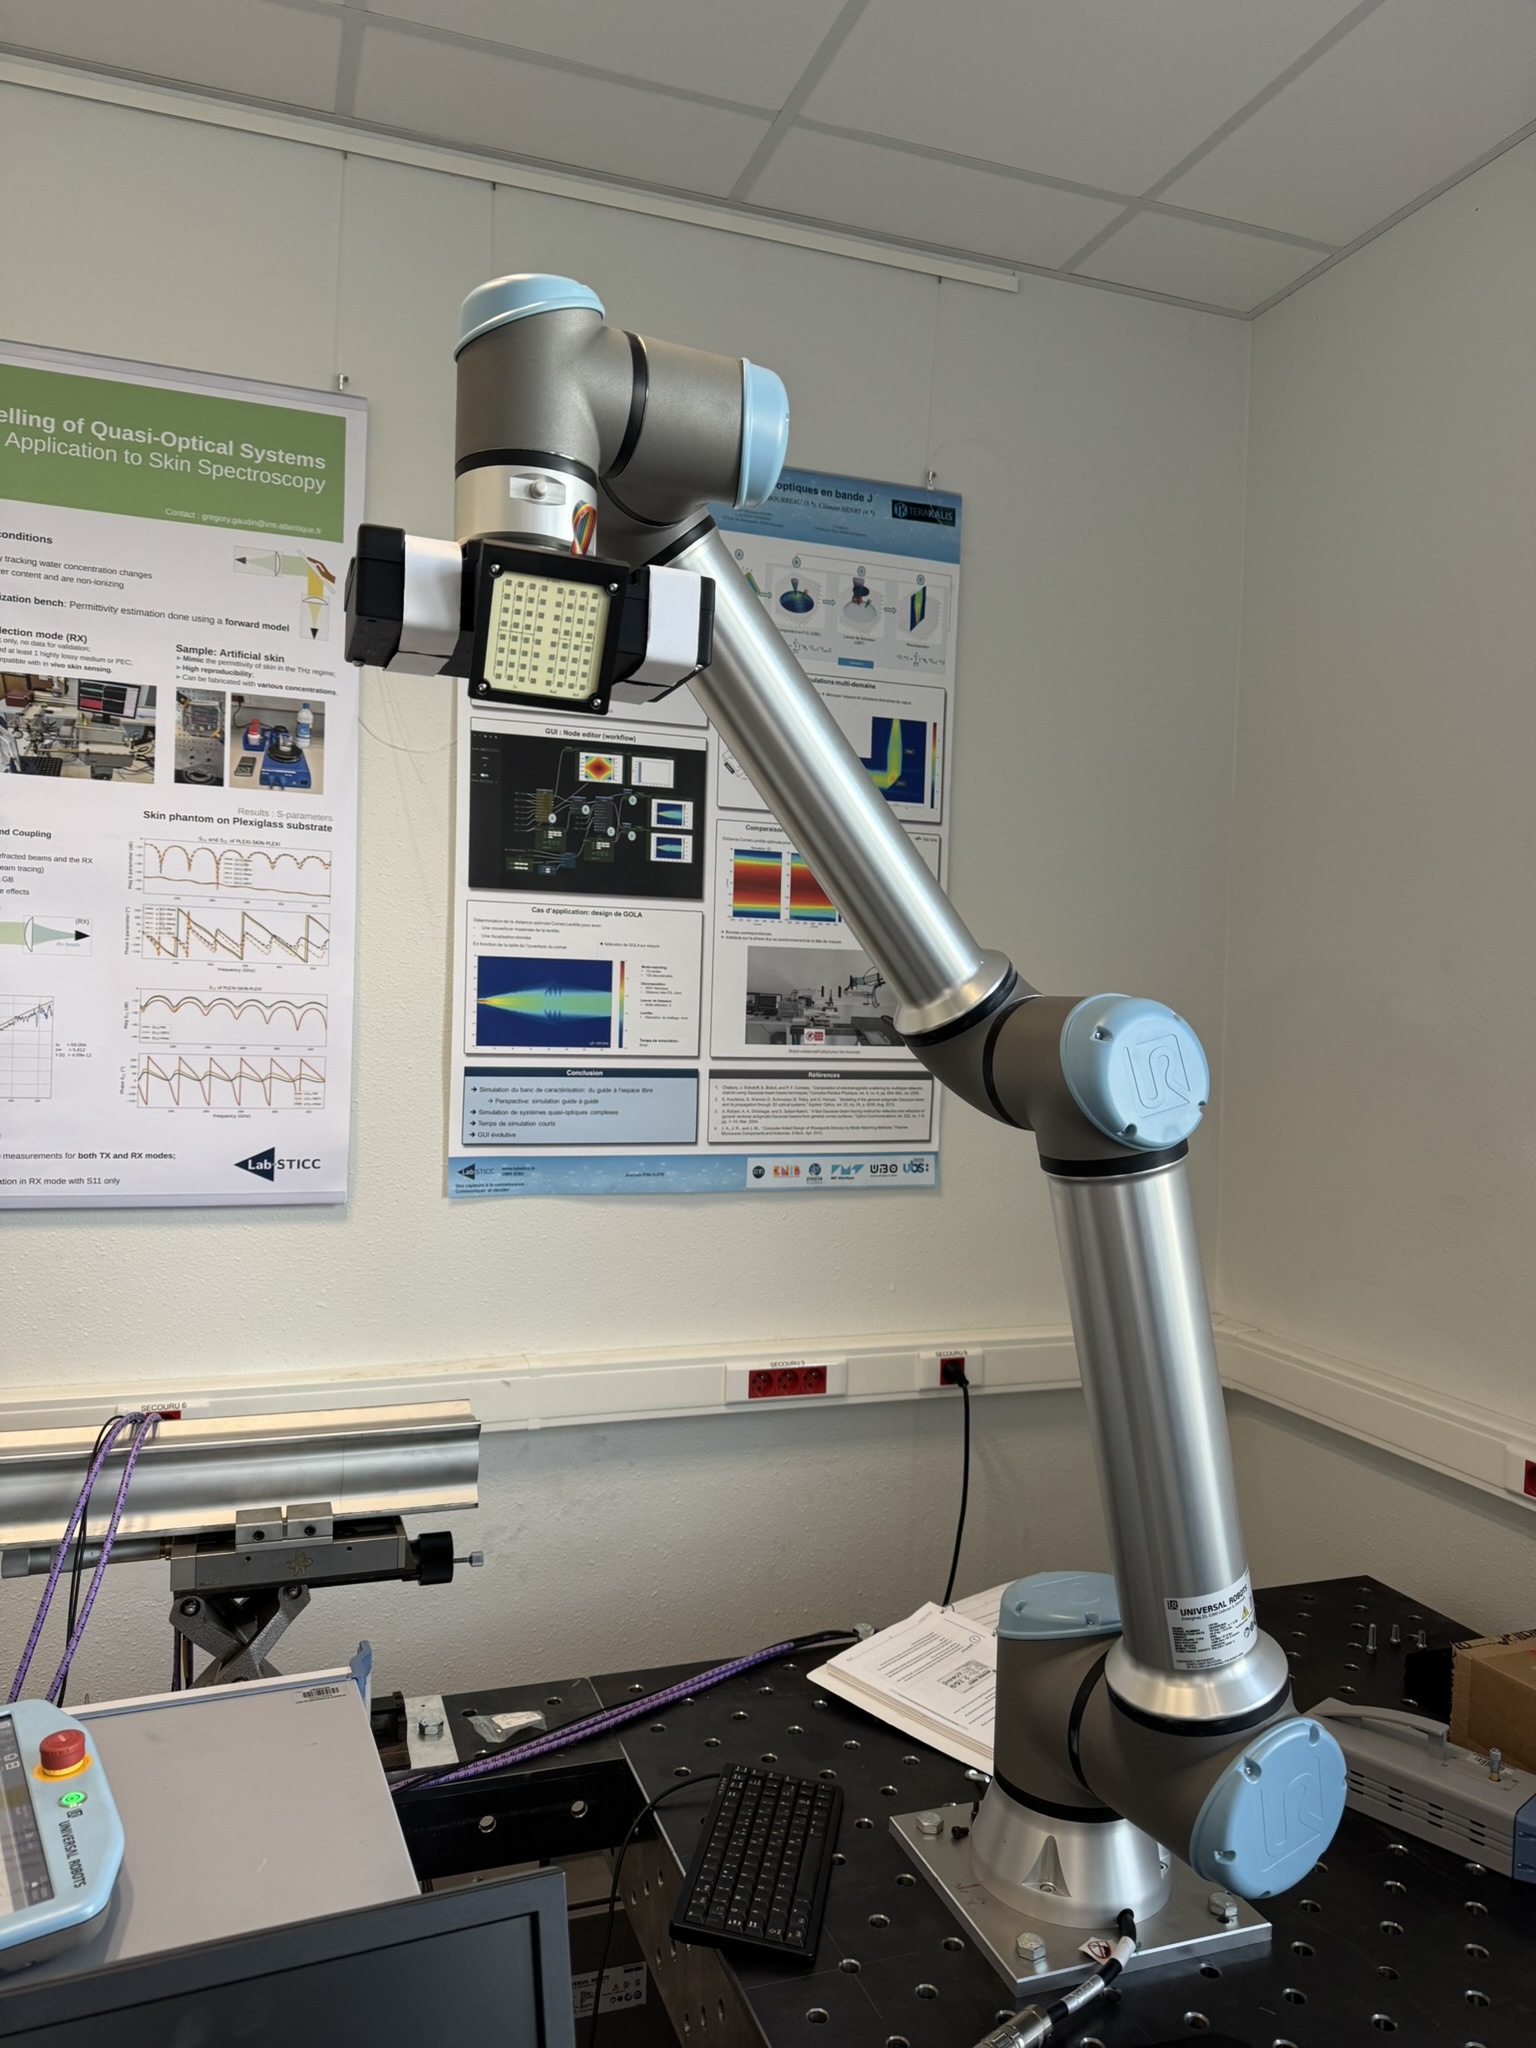
\includegraphics[width=\textwidth]{src/rapport_complet/img/casing_robot.JPEG}
        \caption{Vue de l'assemblage monté sur le robot}
        \label{fig:SARDINE_CASING}
    \end{subfigure}
    
    \caption{Assemblage fabriqué}
    \label{fig:figure_globale}
\end{figure}

\paragraph*{Conclusion}

La conception et la fabrication de ces pièces mécaniques ont permis d’assurer une intégration stable et reproductible du capteur radar et de son antenne, tout en offrant la flexibilité nécessaire à l’adaptation des configurations expérimentales. L’ensemble du dispositif est désormais assemblé et monté sur le bras robotisé, ce qui permet de disposer d’une plateforme expérimentale fonctionnelle.
Les travaux peuvent ainsi se concentrer sur la réalisation des premiers tests expérimentaux en mouvement et sur l’exploitation des données acquises au sein de la chaîne de traitement SAR.